Module manager is useful for creating modular view of large networks without loosing details of modules (using “nest”, object of Cytoscape v7 and after).

\subsection{Create network of modules}
\textbf{Plugins$\Rightarrow$BiNoM module manager$\Rightarrow$Create network of modules}\\
Create a new network from a list of sub-networks (sub-networks are selected in the network list see figure~\ref{Create_network_of_modules}).\\
Nodes=modules, no edge. Visual style created in VizMapper for module network . The got network is as \ref{M-Phase_Material_Modular} without edge and with nodes on grid.\\
\includegraphics[width=12pt,height=12pt]{graphics/warning} Module names and node names must be different, all network names too.\\\\
To go from module to sub-network:\\
select node$\Rightarrow$CRight click$\Rightarrow$CNested Network$\Rightarrow$Go to Nested Network.
\begin{figure}
\centering
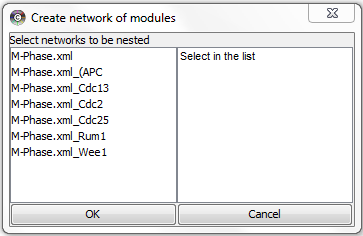
\includegraphics[width=0.8\textwidth]{graphics/Create_network_of_modules}
\caption{Dialog for select networks to become modules in modular0}
\label{Create_network_of_modules}
\end{figure}

\subsection{Create connections between modules}
\textbf{Plugins$\Rightarrow$BiNoM module manager$\Rightarrow$Create connections between modules}\\
Create edges linking modules from all edges of the selected network.\\
Links are simplified, no distinction between left and right (molecule flow), no duplication if same interaction.\\
Warning message if duplicated or absent nodes (may disturb links).
\begin{figure}
\centering
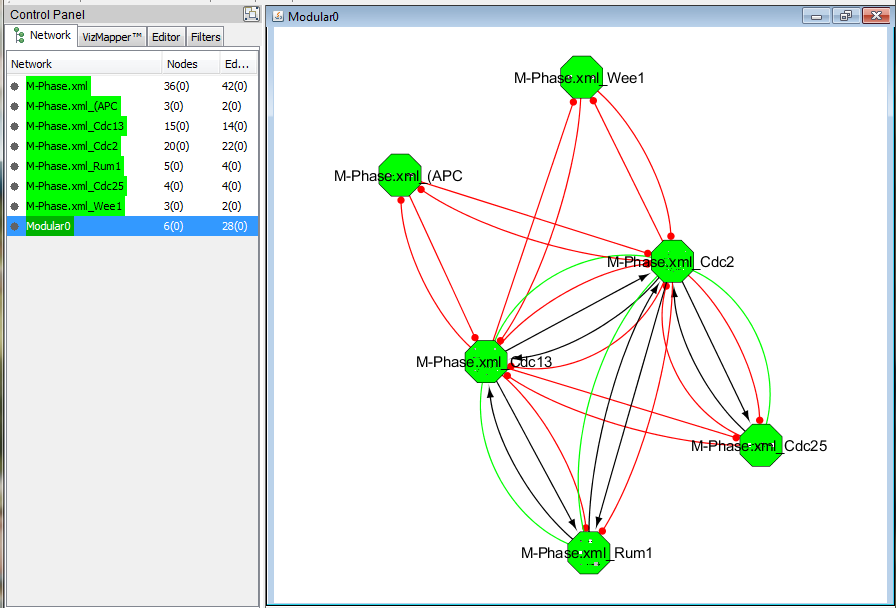
\includegraphics[width=0.8\textwidth]{graphics/M-Phase_Material_Modular}
\caption{M-Phase is divided into modules by get material component. The modular view is got by creating network of modules with organic layout. The function "Create connections between modules" links modules according to the reference network. The function "Find common nodes in modules" creates intersection edges. }
\label{M-Phase_Material_Modular}
\end{figure}

\subsection{Create modules from networks}
\textbf{Plugins$\Rightarrow$BiNoM module manager$\Rightarrow$Create modules from networks}\\
Create modules in the active network from a list of sub-networks (sub-networks are selected in the network list)\\
All edges are kept. See edge attribute PREVIOUS\_ID for their origin.\\
The attribute BIOPAX\_NODE\_TYPE is set to “pathway” (see visual style BiNoM BioPAX).\\
\includegraphics[width=12pt,height=12pt]{graphics/warning} All nodes of sub-networks must be found once in the active network (no intersection between sub-networks).

\subsection{Agglomerate the nearest nodes in modules}
\textbf{Plugins$\Rightarrow$BiNoM module manager$\Rightarrow$Agglomerate the nearest nodes in modules}\\
Create modules and a modular view by agglomerating the nearest nodes in the active network (see~algorithm~in section~\ref{Agglomeration_by_shortest_path}.\\\\
Input 2 parameters to get not too big sub-networks containing not too far nodes:
\begin{itemize}
\item Maximal distance between nodes or modules in number of edges,
\item Maximal number of nodes in modules.
\end{itemize}
Confirm creation if agree with displayed result (see dialog~\ref{Agglomerate_in_modules_dialog}).\\\\
Sub-networks are created and gathered in a packed network as the function "Create modules from networks" (see figure~\ref{M-Phase_packed}).
\begin{figure}
\centering
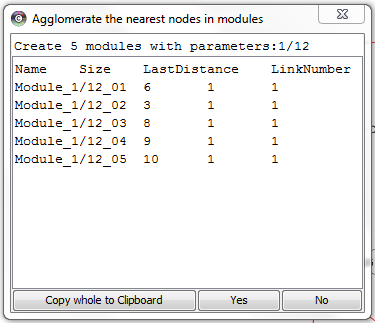
\includegraphics[width=0.8\textwidth]{graphics/Agglomerate_in_modules_dialog}
\caption{This window displays modules, number of node, last distance and number of links of agglomerating process. Yes lauches the process of agglomerating.}
\label{Agglomerate_in_modules_dialog}
\end{figure}
\begin{figure}
\centering
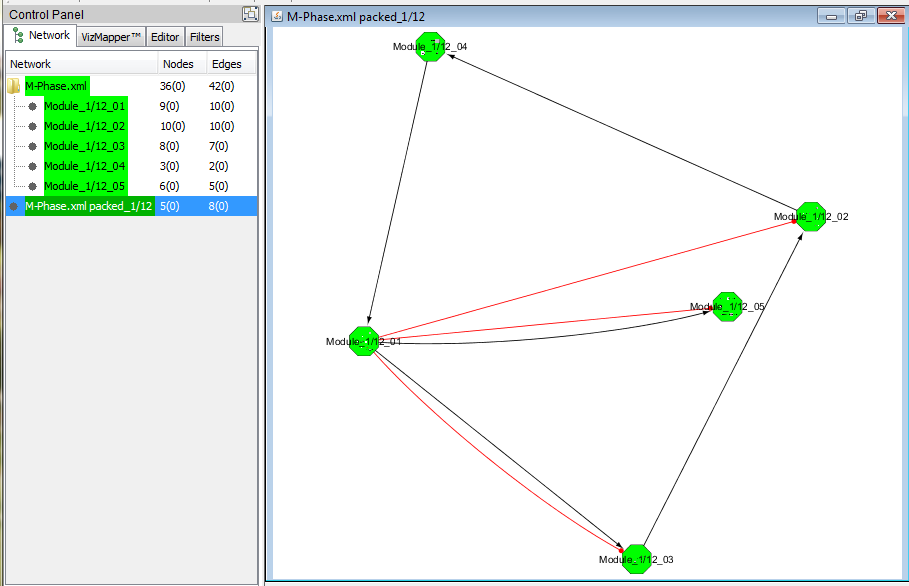
\includegraphics[width=0.8\textwidth]{graphics/M-Phase_packed}
\caption{M-Phase is got by creating network from modules, modules created by agglomerating the nearest nodes (maximal distance=1, maximal size=12 nodes).}
\label{M-Phase_packed}
\end{figure}

\subsection{List nodes of modules and network}
\textbf{Plugins$\Rightarrow$BiNoM module manager$\Rightarrow$List nodes of modules and network}\\
List nodes of network and nodes included in modules.\\
Result in text box can be simply copied in a spreadsheet through clipboard.

\subsection{Find common nodes in modules}
\textbf{Plugins$\Rightarrow$BiNoM module manager$\Rightarrow$Find common nodes in modules}\\
Display in text box the belonging matrix of nodes (modules in columns, nodes in rows, size of modules in last row, frequency in modules in last column); result more easily usable after copying in a spreadsheet (see~\ref{Common_nodes_in_modules}.\\\\
Create intersection edges with number of common nodes as attribute (COMMON\_NODES), green edges in figure~\ref{M-Phase_Material_Modular}.\\\\
Create node attribute containing the node numbers of modules (NODE\_NUMBER).\\\\
Module Visual StyleCan be adapted to the wished visual aspect by hands in VizMapper, for example:
\begin{itemize}
\item To visualize NODE\_NUMBER: double click Node Size, select NODE\_NUMBER, continuous mapping, adjust width by graphical view.
\item To visualize COMMON\_NODES double click Edge Line Width, select COMMON\_NODES, continuous mapping, adjust width by graphical view.
\end{itemize}
\begin{figure}
\centering
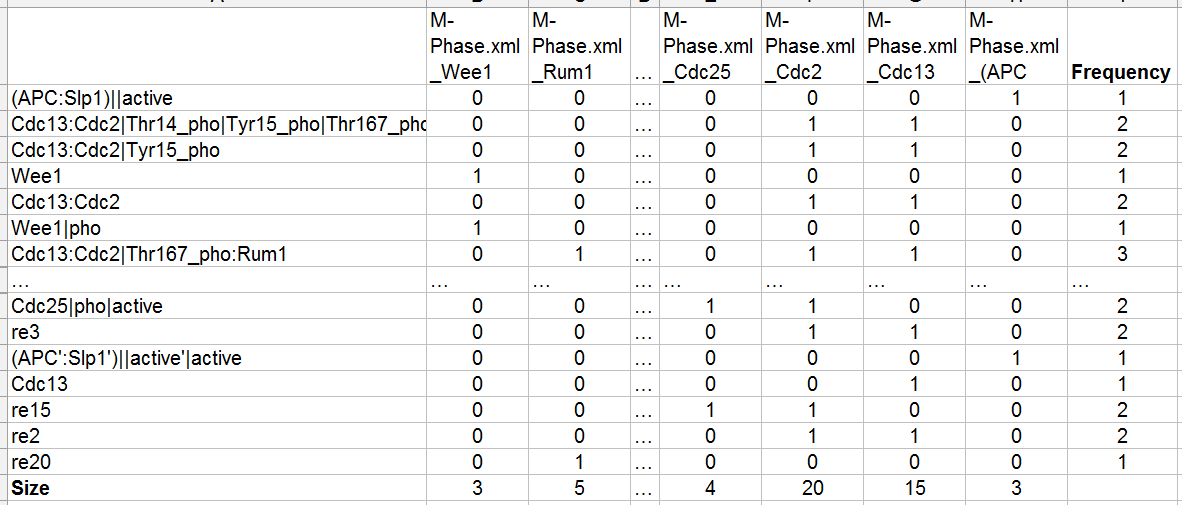
\includegraphics[width=0.8\textwidth]{graphics/Common_nodes_in_modules}
\caption{Matrix of nodes: modules in columns, nodes in rows, size of modules in last row, frequency in modules in last column.}
\label{Common_nodes_in_modules}
\end{figure}

\subsection{Assign module names to node attribute}
\textbf{Plugins$\Rightarrow$BiNoM module manager$\Rightarrow$Assign module names to node attribute}\\
Create a node attribute (named as the modular network), containing module names. This attribute may be used to visualize modules in the reference network.

\subsection{List components of species in network and modules}
\textbf{Plugins$\Rightarrow$BiNoM module manager$\Rightarrow$List components of species in network and modules}\\
List components of species (their names must respect BiNoM syntax). Useful to name modules.

\subsection{Create network from union of selected modules}
\textbf{Plugins$\Rightarrow$BiNoM module manager$\Rightarrow$Create network from union of selected modules}\\
Create a network from union of selected modules and its corresponding module in the current network (named by module names separated by \&).

\subsection{Create network from intersection of 2 selected modules}
\textbf{Plugins$\Rightarrow$BiNoM module manager$\Rightarrow$Create network from intersection of 2 selected modules}\\
Create a network from intersection of 2 selected modules and its corresponding module (named by module names separated by \textbar.\\\\
Confirm for deleting the common nodes in the selected modules.

\subsection{Recreate lost connections inside modules}
\textbf{Plugins$\Rightarrow$BiNoM module manager$\Rightarrow$Recreate lost connections inside modules}\\
Recreate connections inside modules which may have been lost by modularizing operations.

\subsection{Destroy networks unused as module}
\textbf{Plugins$\Rightarrow$BiNoM module manager$\Rightarrow$Destroy networks unused as module}\\
Select networks to be deleted among a list of networks which are not used as modules in the current network (simplify cleaning session).